\documentclass[11pt,a4paper,sans]{moderncv}

% --- 1. ESTILO MODERNCV ---
\moderncvstyle{banking}
\moderncvicons{awesome}

% --- 2. FUENTES ---
\usepackage{fontspec}
\usepackage{geometry}

% Configuración de idioma simplificada para evitar errores de compilación
\usepackage[spanish,es-nodecimaldot,es-tabla,es-noquoting,es-notilde]{babel}

% Definimos Noto Sans como fuente principal
\setmainfont{Noto Sans}
\setsansfont{Noto Sans}
\setmonofont{Noto Sans Mono}

% Definimos una fuente Serif específica para el nombre (Autoridad y Elegancia)
\newfontfamily\headerfont{Noto Serif}

% --- 3. GEOMETRÍA Y GRÁFICOS ---
\geometry{scale=0.88, top=1.5cm, bottom=1.5cm, left=1.2cm, right=1.2cm}
\usepackage{tikz}
\usetikzlibrary{calc, decorations.markings, fadings}
\usepackage{eso-pic}
\usepackage{enumitem}
\usepackage{graphicx} % Requerido para procesar la imagen de perfil

% --- 4. PERSONALIZACIÓN ---
\definecolor{color1}{RGB}{75, 0, 130} % Violeta Fractal
\definecolor{color2}{RGB}{60, 60, 60}
\definecolor{gold}{RGB}{218, 165, 32} % Oro

% Ajuste de fuente para el nombre
\renewcommand*{\namefont}{\fontsize{24}{28}\headerfont\bfseries}

% --- FONDO FRACTAL Y MARCADOR DE FOTO ---
\AddToShipoutPictureBG{
    \begin{tikzpicture}[remember picture, overlay]
        % --- ESPIRAL DE FIBONACCI (Esquina inferior derecha) ---
        \node[opacity=0.15, anchor=south east] at ($(current page.south east) + (2, -2)$) {
            \begin{tikzpicture}[scale=1.8, rotate=90] 
                % Rectángulos Áureos en ORO
                \draw[gold, very thick] (0,0) rectangle (1,1);
                \draw[gold, very thick] (0,1) rectangle (1,2);
                \draw[gold, very thick] (1,0) rectangle (3,2);
                \draw[gold, very thick] (0,-3) rectangle (3,0);
                \draw[gold, very thick] (-5,-3) rectangle (0,5);
                \draw[gold, very thick] (3,-3) rectangle (11,10);
                % Curva Fibonacci en VIOLETA
                \draw[color1, line width=2.5mm, domain=0:4*pi, variable=\t, samples=500, smooth, cap=round]
                    plot ({0.2*exp(0.30635*\t)*cos(\t r + 180)}, {0.2*exp(0.30635*\t)*sin(\t r + 180)});
            \end{tikzpicture}
        };
        
        % --- DETALLE SUPERIOR ---
        \node[opacity=0.1, anchor=north west] at (current page.north west) {
             \begin{tikzpicture}[scale=0.8]
                \draw[gold, thick, domain=0:18, variable=\t, samples=100, smooth]
                    plot ({\t r}: {0.05*exp(0.30635*\t)});
             \end{tikzpicture}
        };
    \end{tikzpicture}
}

% --- DATOS PERSONALES (ESTRATEGIA DE ALINEACIÓN POR CAJAS) ---
\name{\parbox{\textwidth}{\hspace*{4cm}Jesús Antonio De León Reyes}}{}

\title{\parbox{\textwidth}{\hspace*{4cm}Presidente Fundador ANEFF \\ \hspace*{4cm}{\normalfont\small Director de Proyecto Educativo}}}

\address{San Buenaventura, Ixtapaluca, Edo. de México}{}{}

% Datos de contacto alineados (Se elimina la referencia de LinkedIn)
\extrainfo{%
    \parbox{\textwidth}{%
        \hspace*{4cm}% Mismo desplazamiento que el nombre
        \begin{minipage}{\dimexpr\textwidth-4cm\relax} % Bloque de texto para el resto del ancho
            \faMobile*~5547312303 \quad \bullet \quad \faEnvelope~\href{mailto:jesusdeleonreyes027@gmail.com}{jesusdeleonreyes027@gmail.com} \\[0.2em]
            \faFacebook~Jesús Antonio De León Reyes
        \end{minipage}
    }%
}

% --- CONTENIDO ---
\begin{document}

\makecvtitle

% --- INSERCIÓN DE LA FOTO REAL DE PERFIL EN LA ESQUINA SUPERIOR IZQUIERDA ---
\begin{tikzpicture}[remember picture, overlay]
    \node[anchor=north west] at ($(current page.north west) + (1.2cm, -1.2cm)$) {
        \begin{tikzpicture}
            % Dibujamos un contenedor con bordes redondeados y sombra para albergar la imagen
            \begin{scope}
                \clip[rounded corners=10pt] (0,0) rectangle (3.5, 4.5);
                \node[anchor=center] at (1.75, 2.25) {
                    \IfFileExists{IMG_20260127_051656.jpg}{
                        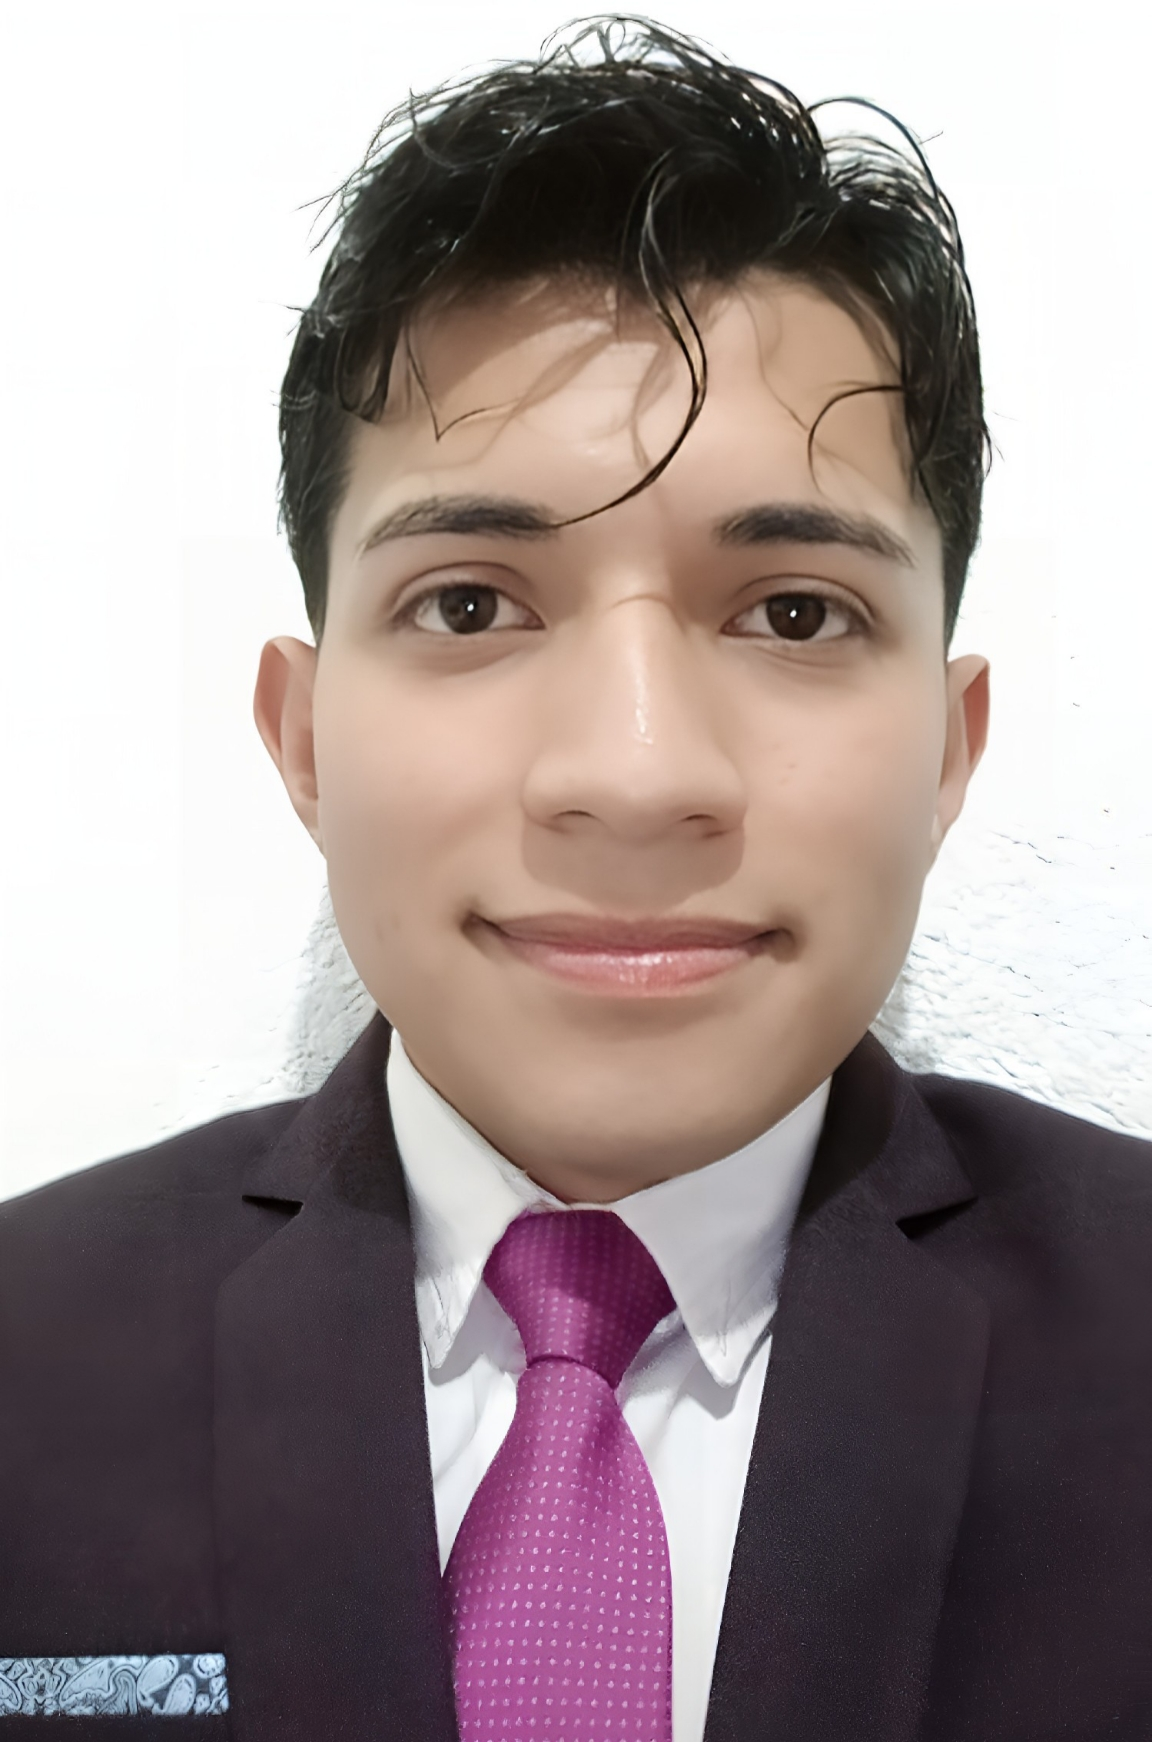
\includegraphics[width=3.5cm, height=4.5cm, keepaspectratio=false]{IMG_20260127_051656.jpg}
                    }{
                        % Respaldo elegante si no detecta el archivo local en el mismo directorio
                        \begin{tikzpicture}
                            \fill[color1!10] (0,0) rectangle (3.5, 4.5);
                            \draw[color1!40, dashed, thick, rounded corners=10pt] (0,0) rectangle (3.5, 4.5);
                            \node[color1!60, align=center] at (1.75, 2.25) {\small\faUser\\ \vspace{0.2cm}\textbf{Añadir Foto}};
                        \end{tikzpicture}
                    }
                };
            \end{scope}
            % Marco exterior refinado en color Violeta Fractal
            \draw[color1, thick, rounded corners=10pt] (0,0) rectangle (3.5, 4.5);
        \end{tikzpicture}
    };
\end{tikzpicture}

\section{Perfil Profesional}
\cvitem{Misión Profesional}{Proveer inteligencia financiera de alto nivel mediante el procesamiento de datos y modelos matemáticos, transformando información compleja en reportes estratégicos escritos que fundamenten la toma de decisiones corporativas y la mitigación de riesgos.}
\cvitem{Visión}{Ser un pilar técnico en la estructura de análisis de la organización, implementando sistemas de evaluación financiera (Web3/Python) que automaticen procesos y garanticen la precisión operativa sin depender de métodos tradicionales de gestión.}

\section{Experiencia Profesional}

% Modificado para dejar únicamente (3º de primaria) en el primer punto
\cventry{2021 -- Presente}{Presidente Fundador / Director de Proyecto}{Asociación Nacional de Educación Financiera Fractal (ANEFF)}{Ciudad de México}{}{
\begin{itemize}
    \item \textbf{Arquitecto del Programa Educativo:} Autor intelectual y gestor de la propuesta ``La Inclusión Fractal'', logrando su incorporación oficial en los libros de texto de la Nueva Escuela Mexicana (3º de primaria) tras ganar el Concurso Nacional de Educación Financiera.
    \item \textbf{Desarrollo de Infraestructura de Datos:} Diseñé e implementé la arquitectura de la red distribuida local utilizando micro-nodos y servidores descentralizados basados en hardware Raspberry Pi bajo sistemas Linux.
    \item \textbf{Gestión Institucional:} Coordinación y comunicación directa con el Presidente de México, Andrés Manuel López Obrador, y la Secretaria de Educación, Delfina Gómez Álvarez, así como organismos aliados (Enseña por México), para la validación y escalabilidad de modelos pedagógicos basados en la naturaleza.
\end{itemize}
}

\section{Habilidades Técnicas (Technical Skills)}

\subsection{1. Análisis de Datos y Tecnología}
\cvitem{Lenguajes}{Python (Enfoque en Ciencia de Datos, Automatización y desarrollo backend con Flask).}
\cvitem{Bases de Datos}{Gestión y estructuración de información (JSON / SQL) para entornos descentralizados y corporativos de persistencia local.}
\cvitem{Blockchain \& Web3}{Desarrollo de contratos inteligentes, arquitectura de tokens (EDUFT) y sistemas de identidad soberana digital (SBT).}

\subsection{2. Finanzas Cuantitativas y Gestión de Riesgos}
\cvitem{Modelado}{Aplicación de geometría fractal, teoría de retículos multidimensionales (Retículo $E_8$) y Sucesión de Fibonacci para proyecciones de mercado.}
\cvitem{Risk Mgmt}{Estrategias de preservación de capital y cálculo de volatilidad y análisis cuantitativo con márgenes de error reducidos.}
\cvitem{Análisis Técnico}{Dominio de Ondas de Elliott y ratios áureos para la identificación de tendencias de mercado.}

\subsection{3. Herramientas y Metodologías}
\cvitem{Ofimática}{Microsoft Excel (Análisis de datos, Tablas dinámicas y Reportes ejecutivos).}
\cvitem{Dev \& IoT}{Dominio de Visual Studio Code (VS) para gestión de código, integrando despliegue de nodos y optimización de recursos en Raspberry Pi.}
\cvitem{Gestión}{Metodologías Ágiles para el desarrollo de productos eficientes.}

\section{Formación Académica}
\cventry{2020}{Curso de Trading con Fractales ``Alpha''}{VIBLO}{Modalidad Asincrónica}{}{Token Viblo}
\cventry{2014 -- 2016}{Bachillerato General}{EPOEM 141 ``Leones Blancos''}{San Buenaventura, Edo. Méx.}{}{}

\section{Certificaciones y Reconocimientos}

\cvitem{Mérito Educativo}{\textbf{1er Lugar Nacional (Enseña por México):} Por el ensayo ``La inclusión fractal en el sistema educativo; un futuro global de cambio universal''.}

\subsection{Banco Santander X}
\begin{itemize}
    \item \textbf{Inteligencia Artificial}
    \item \textbf{Estrategia Corporativa}
    \item \textbf{Liderazgo y Talento}
    \item \textbf{Gestión y Operaciones}
    \item \textbf{Growth \& Ciberseguridad}
    \item \textbf{Tecnología e Innovación}
    \item \textbf{Finanzas y Negocios}
\end{itemize}

\end{document}
